\documentclass[tikz,border=2mm]{standalone}
\usetikzlibrary{arrows.meta}

\begin{document}
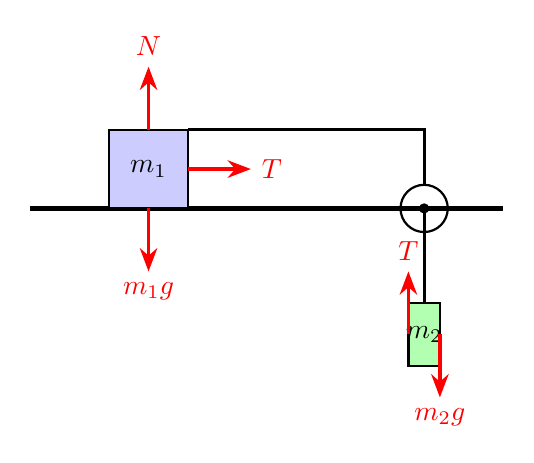
\begin{tikzpicture}[scale=1, thick, 
    force/.style={->, red, very thick, >=Stealth}]

% Table
\draw[line width=2pt] (0,0) -- (6,0);

% Block m1 on the table
\draw[fill=blue!20] (1,0) rectangle (2,1);
\node at (1.5,0.5) {$m_1$};

% Pulley
\draw (5,0) circle (0.3);
\draw[fill=black] (5,0) circle (0.05);

% Hanging block m2
\draw[fill=green!30] (4.8,-2) rectangle (5.2,-1.2);
\node at (5,-1.6) {$m_2$};

% String
\draw[line width=1pt] (2,1) -- (5,1) -- (5,0.3);
\draw[line width=1pt] (5,-1.2) -- (5,0);

% Forces on m1
\draw[force] (1.5,1) -- (1.5,1.8) node[above] {$N$};
\draw[force] (1.5,0) -- (1.5,-0.8) node[below] {$m_1 g$};
\draw[force] (2,0.5) -- (2.8,0.5) node[right] {$T$};

% Forces on m2
\draw[force] (5.2,-1.6) -- (5.2,-2.4) node[below] {$m_2 g$};
\draw[force] (4.8,-1.6) -- (4.8,-0.8) node[above] {$T$};

\end{tikzpicture}
\end{document}